Eines der Hauptthemen der Diplomarbeit war die Überarbeitung des bisherigen Designs. 
Um dies zu erreichen, wurden nicht nur über die aktuellen Standards und Trends analysiert, 
der aktuelle Content der Website restrukturiert und Usability-Tests durchgeführt, 
sondern auch ein mehrstündiger Workshop zum Thema UI/UX Design an der JKU absolviert.

\section{Analyse}
\setauthor{Mona Angerer}
Um ein umfassendes Verständnis für die derzeit gängigen Designmethoden erhalten zu können, wurden zahlreiche bekannte große Websites wie die von Apple und anderen analysiert.
Dabei wurden die überschneidenden Merkmale identifiziert und herausgearbeitet und diejenigen, die für die HTL-Website besonders relevant sind, anschließend genauer untersucht. 
Auffällig ist dabei die übergeordnete Präferenz für das Motto „Weniger ist mehr“. Durchgehend dominiert minimalistisches Design mit vielen weißen Flächen, wodurch ein edler, strukturierter Eindruck erweckt wird.

Im Kontrast dazu werden jedoch auch viele Vektor- oder svg-Animationen, oftmals auch im „handgezeichneten“ Stil, verwendet, die das saubere Layout auflockern und Bewegung in die Benutzeroberfläche bringen. 

Darüber hinaus gewinnen Scrollingeffekte zunehmend an Bedeutung und werden von immer mehr Unternehmen als wichtiges und vielseitig einsetzbares Designelement betrachtet. 
Ob Parallax-Effekte, Scrollitelling, Immersive oder Horizontal Scrolling – das Weiterscrollen wird nicht mehr nur als „Bildschirminhalt verschieben“ gesehen, 
sondern wird zu einem immer wichtigeren, vielseitig eingesetzten Element. 

Ein weiterer interessanter Trend ist die verstärke Aufmerksamkeit auf individuell gestaltete
Error-Seiten. Diese werden zunehmend in das Gesamtdesign der Website integriert und mit kleinen 
Spielereien wie Animationen oder Mini-Games ausgeschmückt. 

Geometrische Ästhetik, insbesondere abstrakte Formen wie Dreiecke, 
Kreise, Vierecke oder eine Kombination davon, gewinnen im Web-Bereich deutlich sichtbar an Popularität. 
Auf vielen hochwertigen Websites tragen diese geometrischen Gestaltungselemente dazu bei, eine strukturierte und interessante Oberfläche zu schaffen. 


\section{Content-Strukturierung}
\setauthor{Mona Angerer}
Durch Gespräche mit SchülerInnen, Lehrkräften und InteressentInnen fand man hinaus, dass einer der am häufigsten bemängelten Aspekte der bisherigen 
HTL-Website der unübersichtliche Aufbau mit etlichen Unterseiten ist. Es fiel den Usern teilweise schwer, sich auf der Benutzeroberfläche zu orientieren 
und den gesuchten Inhalt auf Anhieb zu finden. Um dieses Problem anzugehen, wurde zunächst eine eingehende Analyse des Menüs und seiner Unterpunkte durchgeführt, 
um einen umfassenden Überblick über den gesamten Website-Inhalt zu erhalten. Nach intensiver Prüfung wurde festgestellt, dass durch eine Neustrukturierung von 
7 Menüpunkten auf nur noch 5 Hauptseiten übergegangen werden könnte.

Des Weiteren wurde ein erheblicher Teil des Inhalts von der Website ins LeoWiki, das interne Wiki der HTL Leonding, ausgelagert. 
Dies verhindert, dass Content, der nur für Personen, die bereits an der HTL Leonding lernen oder lehren, relevant ist, für Außenstehende sichtbar ist und ermöglicht, 
dass die meisten Seiten keine weiteren Unterseiten besitzen und somit als One Pager fungieren, auf denen der Inhalt durch einfaches Scrollen zugänglich ist.



\section{Workshop}
\setauthor{Mona Angerer}
An dem Workshop auf dem Campus der JKU, der von … von der Firma KBC abgehalten wurde, nahmen beiden Diplomarbeitsteams, der Betreuungslehrer Herr Professor Huemer und die beiden Professorinnen 
Frau Engleitner und Frau Rammelmüller teil. 

Um einen Ausgangspunkt für die Entwicklung eines Designkonzepts zu schaffen, 
wurde zunächst eine umfassende Problemanalyse durchgeführt. In Teams wurde die bewährte Post-It-Methode angewendet, 
bei der jeder/jede TeilnehmerIn unterschiedlich farbige Zettel erhält, um Mängel und Verbesserungsvorschläge auf gemeinsame Plakate zu kleben. 
Dieser kollaborative Ansatz ermöglichte die Erstellung einer Art Mindmap, auf der die Schwächen der aktuellen HTL-Website deutlich herausgearbeitet wurden. 
Dabei wurden Herausforderungen wie die Unübersichtlichkeit des Menüs, eine zu bunte Gestaltung und Probleme im Mobile-Modus hervorgehoben. 
Diese Methode lenkte den Fokus von Anfang an auf die Lösungsfindung in Beachtung der bereits existierenden Probleme, um somit nicht nur eine Neuimplementierung, 
sondern eine konkrete Verbesserung der Website zu erreichen.

\begin{figure}
    \begin{minipage}[b]{.4\linewidth} 
       \includegraphics[width=\linewidth]{pics/problemanalyse.jpg}
       \caption{Problemanalyse}
    \end{minipage}
    \hspace{.05\linewidth}
    \begin{minipage}[b]{.4\linewidth}
       \includegraphics[width=\linewidth]{pics/zielgruppenanalyse.jpg}
       \caption{Zielgruppenanalyse}
    \end{minipage}
 \end{figure}

Der kreative kollaborative Prozess setzte sich fort und mündete in einer detaillierten Zielgruppenanalyse. 
Dieser Schritt ist von besonderer Bedeutung in der Designentwicklung, da eine Benutzeroberfläche erst dann als gelungen betrachtet werden kann, 
wenn sie von den BenutzerInnen intuitiv genutzt werden kann und ihren individuellen Anforderungen gerecht wird. 
Bei der HTL-Website wurden verschiedene Benutzergruppen identifiziert, darunter SchülerInnen, LehrerInnen, InteressentInnen, Firmen und Eltern. 
Zusätzlich wurden deren spezifische Intentionen berücksichtigt. Beispielsweise ist für Unternehmen von großem Interesse, 
welche Projekte an der Schule verfolgt werden und welche Technologien dafür verwendet werden. 
Eltern und InteressentInnen wiederum möchten vorrangig Informationen zu den angebotenen Zweigen und Fächern an der HTL erhalten, 
während Lehrkräfte und SchülerInnen insbesondere anstehende Events und Aktivitäten im Blick haben möchten. 
Diese präzise Zielgruppenanalyse bildet die Grundlage für ein benutzerzentriertes Designkonzept, das den Bedürfnissen aller Zielgruppen gerecht wird.


Um die Benutzerperspektive noch intensiver zu erfassen, wurde im weiteren Verlauf darauf eingegangen, 
welche Gedanken, Wünsche, Handlungen und Emotionen die NutzerInnen während der Verwendung der Website durchlaufen. 
Dabei wurden nicht nur positive Gefühle und Gedanken, wie Vorfreude und Neugierde, herausgearbeitet, sondern auch potenzielle Ängste oder Unsicherheiten. 
Hierzu gehören beispielsweise Fragen wie: \glqq Bin ich gut genug für die HTL?\grqq oder \grqq Habe ich überhaupt Chancen, aufgenommen zu werden?\grqq.

\begin{figure}
    \begin{minipage}[b]{.4\linewidth} 
       \includegraphics[width=\linewidth]{pics/user_gefühle_gedanken.JPG}
       \caption{User Gefühle}
    \end{minipage}
    \hspace{.05\linewidth}
    \begin{minipage}[b]{.4\linewidth}
       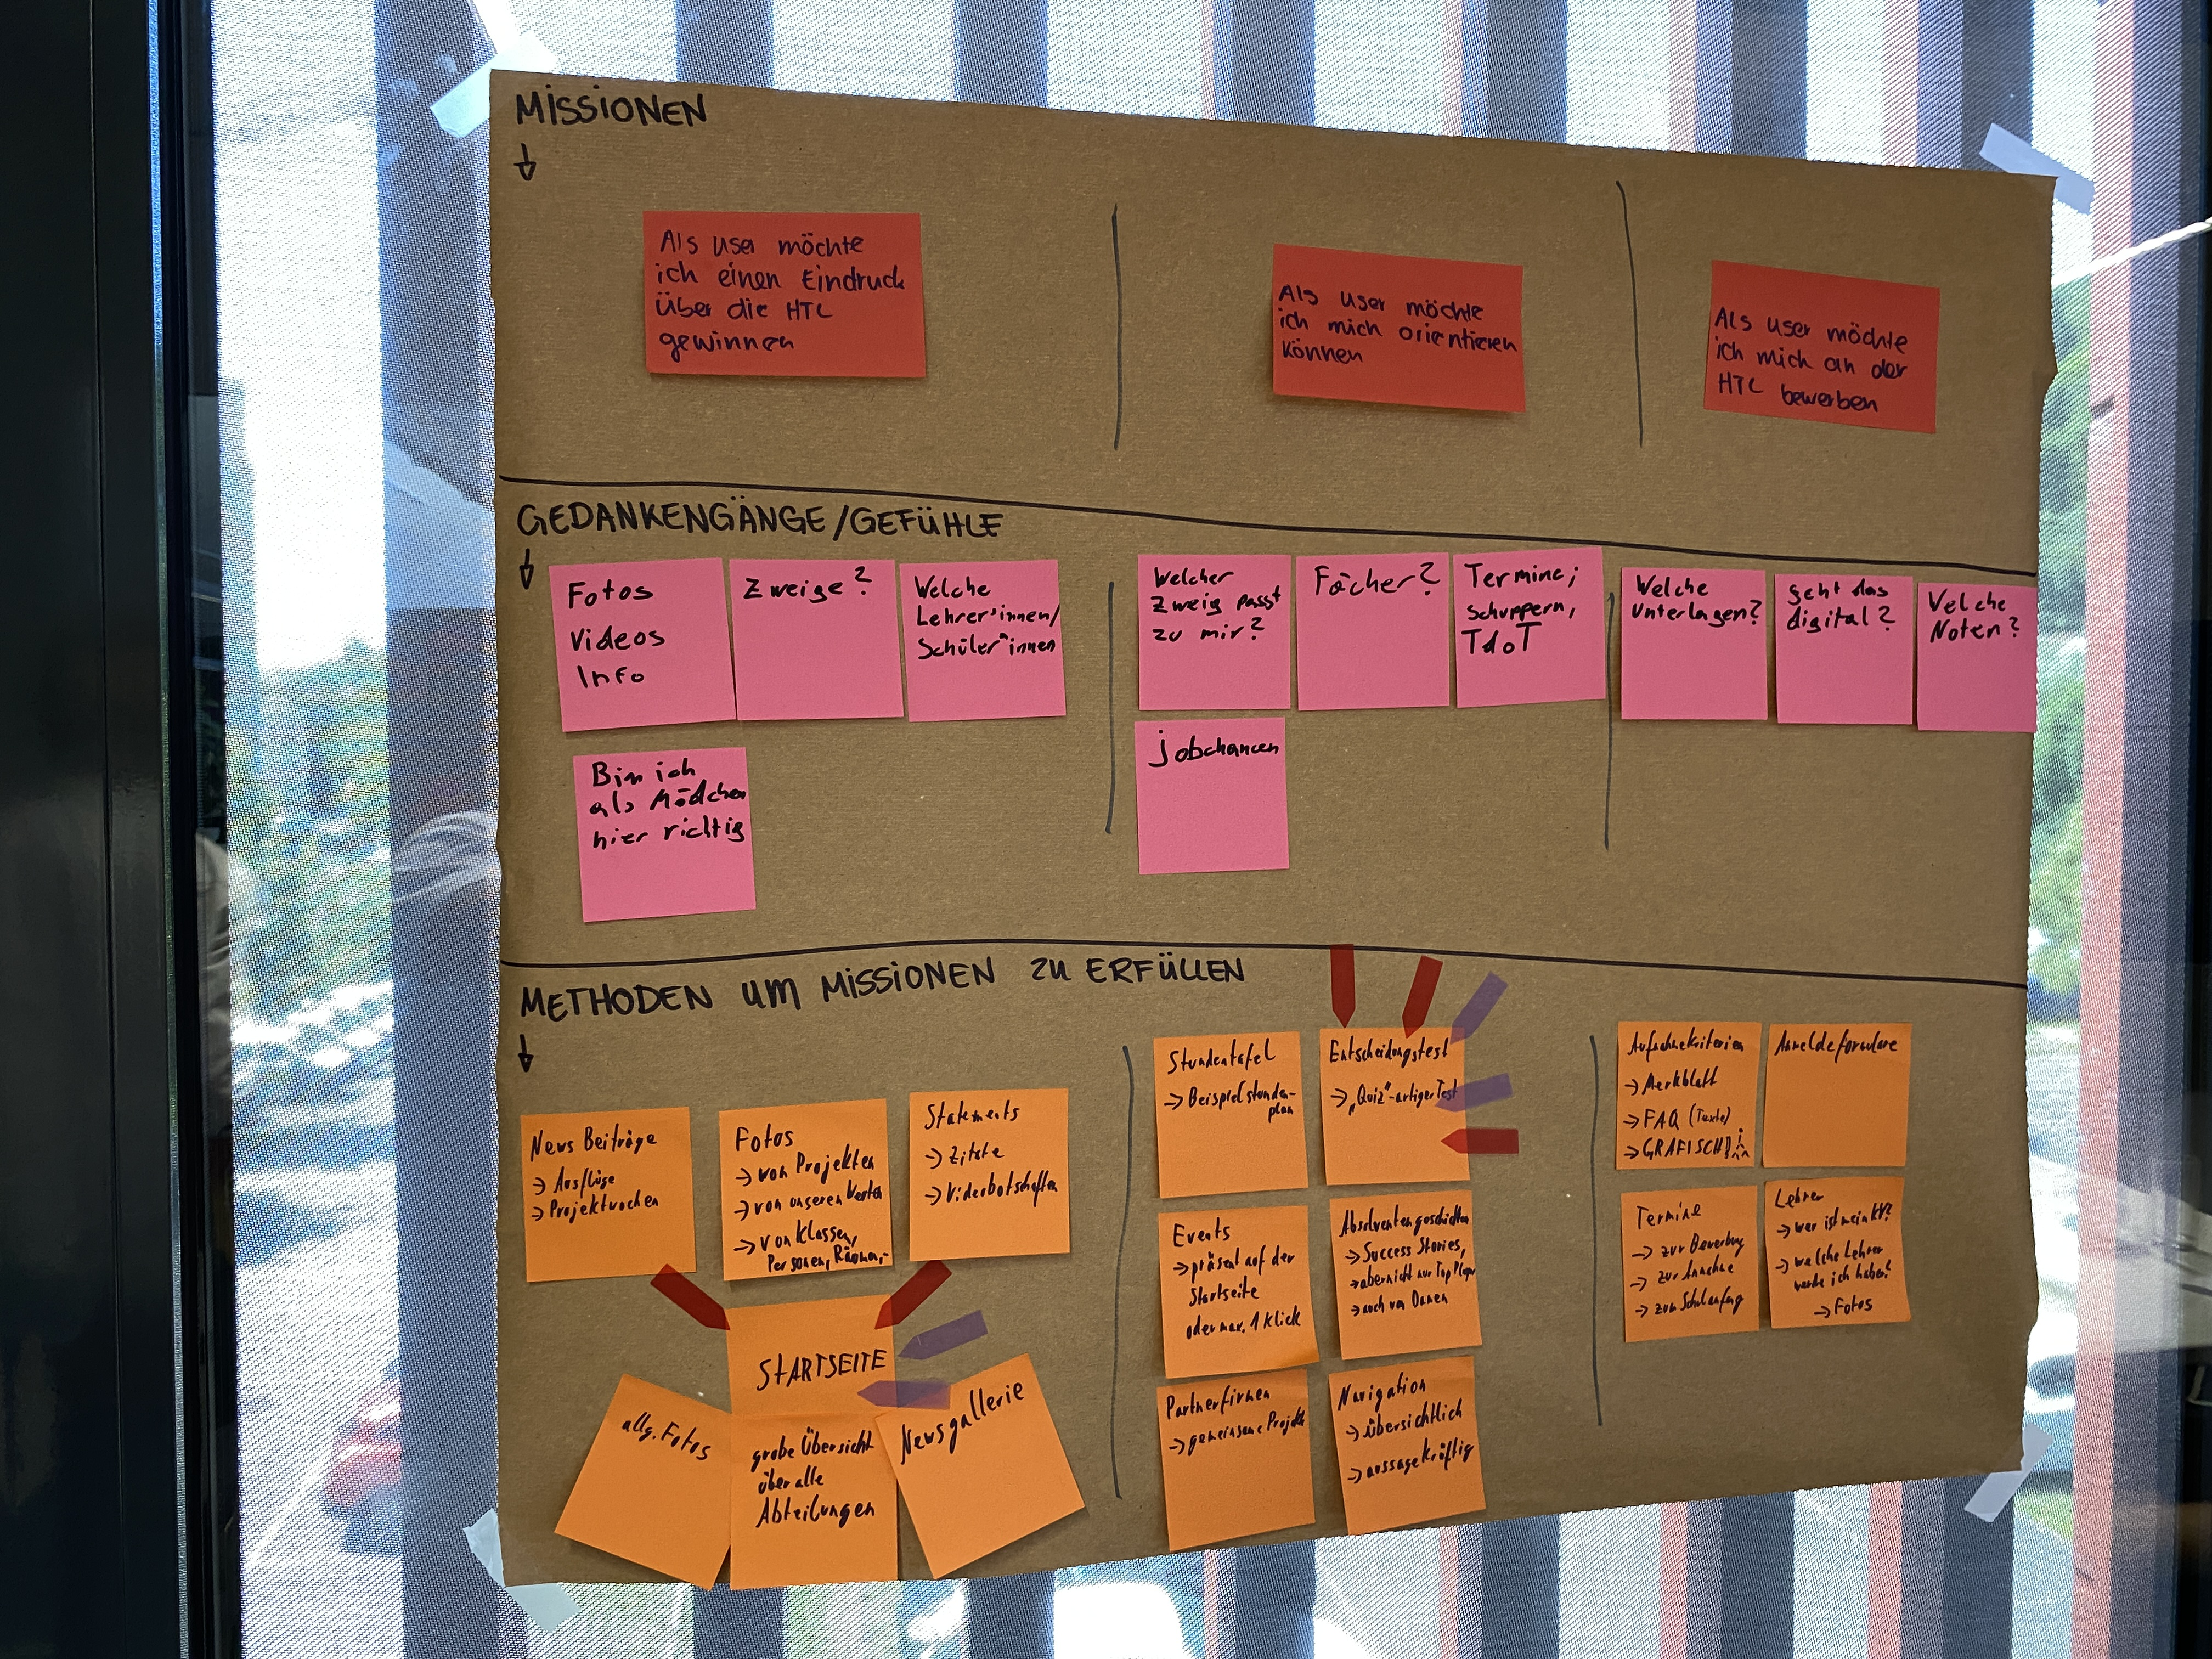
\includegraphics[width=\linewidth]{pics/user_missionen.JPG}
       \caption{User Missionen}
    \end{minipage}
 \end{figure}

Die Berücksichtigung dieser vielschichtigen Nutzererfahrungen ermöglicht eine empathische Gestaltung der Benutzeroberfläche, 
die nicht nur informativ ist, sondern auch dazu beiträgt, positive Emotionen zu fördern und mögliche Ängste zu mildern. 
Durch diese eingehende Analyse der Nutzerperspektive wird die HTL-Website nicht nur funktional, sondern auch emotional ansprechend und unterstützend gestaltet.

Um eine intuitive Benutzererfahrung auf der Website sicherzustellen, wurden darüber hinaus potenzielle Missionen, 
Gedankengänge und Vorgehensweisen der NutzerInnen berücksichtigt, die sie bei ihrem Besuch auf dem HTL-Webauftritt haben könnten. 
Es wurde dabei analysiert, welche konkreten Ziele sie verfolgen, welche Informationen sie suchen und welche Schritte sie wahrscheinlich unternehmen möchten.

Diese detaillierte Betrachtung der Nutzerinteraktion ermöglicht es, die Benutzeroberfläche so zu gestalten, dass sie den natürlichen Denk- und Handlungsmustern 
der BenutzerInnen entspricht. Durch das Verstehen der potenziellen Missionen und Gedankengänge wird sichergestellt, dass die Website nicht nur informativ ist, 
sondern auch nahtlos in den individuellen Ablauf der NutzerInnen integriert wird. Dieser Ansatz fördert eine reibungslose und effektive Nutzung der Website.

Mit dem erlangten Wissen über die zu behebenden Probleme und die unterschiedlichen Usergruppen, deren individuelle Anforderungen 
an die HTL-Website, die Ziele, die sie mit dem Besuch der Website verfolgen möchten und die Emotionen und Eindrücke, die man in den Usern beim benutzen der Oberfläche erwecken will,
wird nun der Startpunkt für die Erstellung eines Designentwurfs erleichtert. Dazu wurde unter den
TeilnehmerInnen des Workshops Zettel und Stifte ausgeteilt, um Skizzen und mögliche Layouts für die Weboberfläche zu gestalten. 
Durch diese Methode werden eine Vielzahl an Ideen erbracht, die in der gesamten Gruppe geteilt und diskutiert werden. 
Dieser kreative Ansatz ermöglicht es, die gewonnenen Erkenntnisse 
unmittelbar in konkrete visuelle Konzepte umzusetzen und so den Grundstein für eine optimierte HTL-Website zu legen.


\section{Usability-Tests}
\setauthor{Mona Angerer}

Nach umfassenden Analysen und Untersuchungen der geeigneten Gestaltungselemente, Effekte und Animationen für die HTL-Website wurde unter Anwendung des im Workshop 
erworbenen Wissens und der Designmethoden ein erster Entwurf erstellt. Die Gestaltung wurde mithilfe der Plattform Figma in Form eines 
Click-Dummies skizziert. Anschließend wurde dieser Entwurf SchülerInnen der ersten und zweiten Klasse der HTL sowie Lehrkräften 
und externen Personen präsentiert. Diese Form der Testung ermöglicht es, direktes Feedback und Bewertungen zu sammeln, um den Entwurf 
weiter zu verfeinern und optimal an die Bedürfnisse der BenutzerInnen anzupassen. Der Prozess integriert somit gezielt die Perspektiven 
der verschiedenen Zielgruppen, um eine benutzerfreundliche Website zu gewährleisten. 
Die erhaltenen Rückmeldungen bekräftigten die verbesserte Struktur und die aufgewertete Anordnung durch die Reduzierung der Menüpunkte. 
Zudem wurde bestätigt, dass die Navigation auf der Benutzeroberfläche merklich vereinfacht wurde. Allerdings wurden auch einige Anregungen 
und Kritiken geäußert, darunter die Empfehlung, vermehrt Schülerfotos einzubinden, um die Website persönlicher zu gestalten. Diese Maßnahme 
soll dazu beitragen, ein einladenderes Bild der HTL Leonding zu vermitteln. Auch wurden einige Verschiebungen von Inhalt in andere Menüpunkte 
vorgeschlagen, um eine logischere Anordnung sicherzustellen. 
Nach der Implementierung dieser Verbesserungsvorschläge wurde der Prozess mehrfach wiederholt, um das Design weiter zu perfektionieren und 
eine optimale Zufriedenheit aller BenutzerInnen sowie eine intuitive Steuerung der Website zu erreichen. 
